\documentclass{article}
\usepackage[utf8]{inputenc}

\title{Path of Exile}
\author{João Pedro Henrique}
\date{April 2019}

\usepackage[colorlinks=true,allcolors=blue]{hyperref}
\usepackage{natbib}
\usepackage{graphicx}

\begin{document}

\maketitle

\section{Introduction}
Path of Exile é um jogo indie desenvolvido pela empresa neozelandesa Grinding Gear Games. Bastante inspirado em Diablo, o jogo surgiu como uma alternativa gratuita ao famoso jogo da Blizzard, e rapidamente se popularizou através da Steam. \cite{poe}

O jogo permite você criar seu personagem com uma classe fixa e construa uma build com habilidades e especialidades a seu critério.

\begin{figure}[h!]
\centering
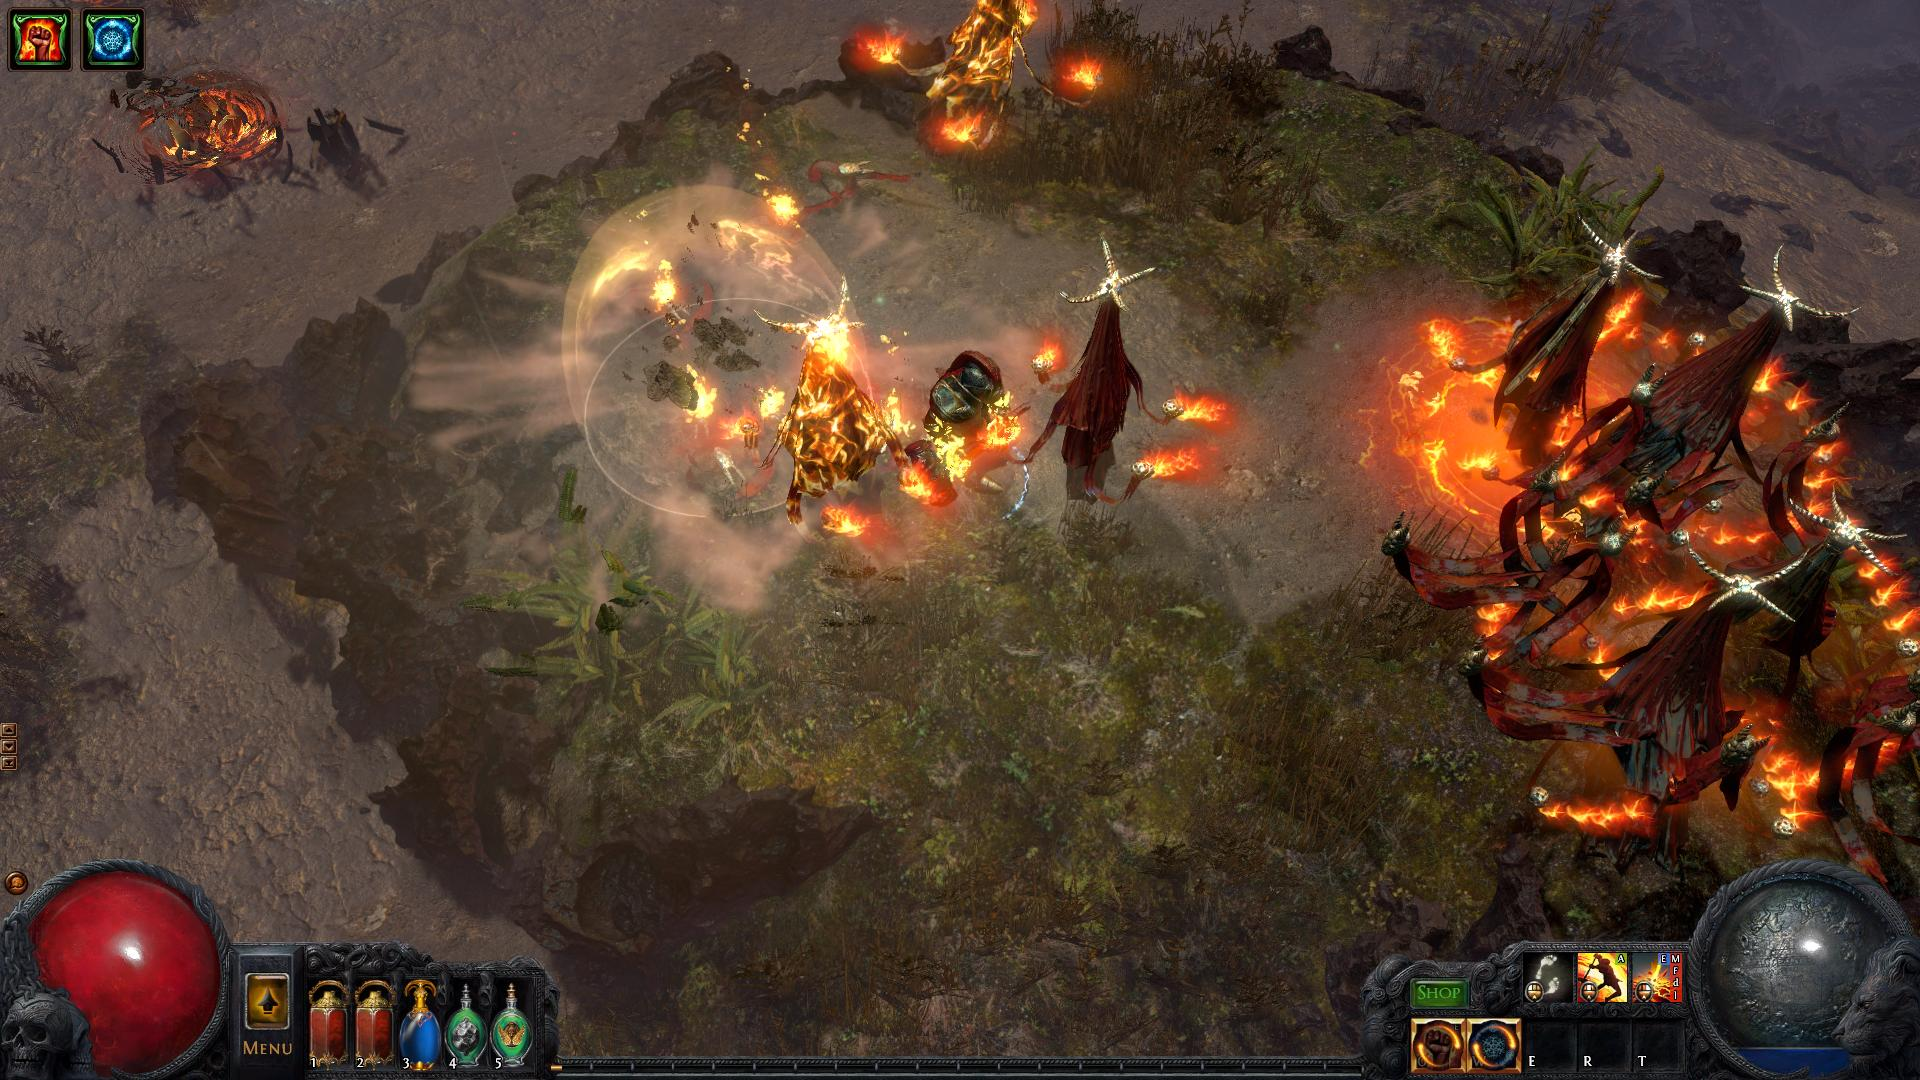
\includegraphics[scale=0.15]{path-of-exile}
\caption{Screenshot de Path of Exile.}
\label{fig:universe}
\end{figure}

\section{Vantagens e Desvantagens}
\subsection{Vantagens}
\begin{itemize}
    \item Gratuito.
    \item Oferece várias possibilidades para a construção do personagem.
    \item Sistema de microtransações. Gastar dinheiro não vai te dar uma vantagem no jogo.
\end{itemize}

\subsection{Desvantagens}
\begin{itemize}
    \item Relativamente pesado.
    \item Jogabilidade complexa para tirar o máximo do jogo.
    \item Algumas coisas são desbalanceadas.
\end{itemize}

\section{Comparações}

\begin{table}[h!]
\begin{tabular}{|l|l|l|}
\hline
             & PoE & Diablo 3 \\ \hline
Jogabilidade & 9   & 9        \\ \hline
Comunidade   & 7   & 8        \\ \hline
Diversidade  & 10  & 10       \\ \hline
\end{tabular}
\end{table}

\bibliographystyle{plain}
\bibliography{references}
\end{document}
